\documentclass[a4paper, 14pt]{extarticle}

\usepackage[T2A]{fontenc}
\usepackage{natbib}
\usepackage{graphicx}
\usepackage[english, russian]{babel}
\usepackage{fontspec}
\usepackage{amsmath}
\usepackage{amsfonts}
\usepackage{amssymb}
\usepackage{amsthm}
\usepackage{mathtools}
\usepackage{mathrsfs}
\usepackage{fullpage}
\usepackage{ulem}
\usepackage{setspace}
\usepackage{listings}
\usepackage{indentfirst}
\usepackage[left=2cm,right=1.5cm,top=2cm,bottom=2cm]{geometry}
\usepackage{xcolor}
\usepackage{float}
\usepackage{csquotes}
\usepackage{hyperref}
\usepackage{graphics}

\definecolor{urlcolor}{HTML}{0000FF} % цвет ссылок
\definecolor{linkcolor}{HTML}{000000} % цвет гиперссылок
\hypersetup{pdfstartview=FitH, linkcolor=linkcolor, urlcolor=urlcolor, colorlinks=true}

\setmainfont{Times New Roman}
\setlength{\parindent}{5ex}
\setlength{\parskip}{1em}
\renewcommand{\baselinestretch}{1}

\graphicspath{{resources/Images}}

\definecolor{buzzlightyear}{HTML}{8757A5}
\definecolor{grass}{HTML}{738D06}
\definecolor{literal}{HTML}{F18A2B}
\definecolor{commentcolor}{HTML}{8E908B}

\lstdefinestyle{habrstyle}{
    backgroundcolor=\color{white},
    commentstyle=\color{commentcolor},
    keywordstyle=\bfseries\color{buzzlightyear},
    numberstyle=\tiny\color{commentcolor},
    stringstyle=\color{grass},
    basicstyle=\ttfamily\footnotesize,
    breakatwhitespace=false,
    breaklines=true,
    captionpos=b,
    keepspaces=true,
    numbers=left,
    numbersep=5pt,
    showspaces=false,
    showstringspaces=false,
    showtabs=false,
    tabsize=4
}

\lstset{style=habrstyle}

\begin{document}
% Титульный лист
    \begin{center}
        \begin{center}
            \hfill \break
            \normalsize{Санкт-Петербургский государственный политехнический}\\
            \normalsize{университет Петра Великого}\\
            \hfill \break
            \normalsize{\textbf{Высшая школа интеллектуальных систем и}}\\
            \normalsize{\textbf{суперкомпьютерных технологий}}\\
            \hfill \break
            \hfill \break
            \hfill \break
            \normalsize{Отчёт по лабораторной работе №1}\\
            \normalsize{Дисциплина: Телекоммуникационные технологии}\\
            \normalsize{Тема: Звуки и сигналы}\\
        \end{center}
        \hfill \break
        \hfill \break
        \hfill \break
        \hfill \break
        \hfill \break
        \hfill \break
        \hfill \break
        \hfill \break
        \hfill \break
        \hfill \break
        \begin{tabbing}
            Выполнил студент гр. 3530901/80201 \`В.А. Пучкина\\
            \\
            Преподаватель: \`Н.В. Богач\\
        \end{tabbing}
        \hfill \break
        \hfill \break
        \hfill \break
        \hfill \break
        \begin{center}
            Санкт-Петербург\\
            2021
        \end{center}
        \thispagestyle{empty}
    \end{center}

% Оглавление
    \newpage
    \tableofcontents

% Список иллюстраций
    \newpage
    \listoffigures

% Список листингов
    \newpage
    \lstlistoflistings

% ---------------------------------------------- Упражнение 1.1 ----------------------------------------------
    \newpage
    \section{Упражнение 1.1}
    \label{sec:task1}

    Загрузим файл \texttt{chap01.ipynb}, изучим его, прочитаем пояснения и запустим примеры.
    Проверим, что всё работает корректно.

    \begin{figure}[h]
        \centering
        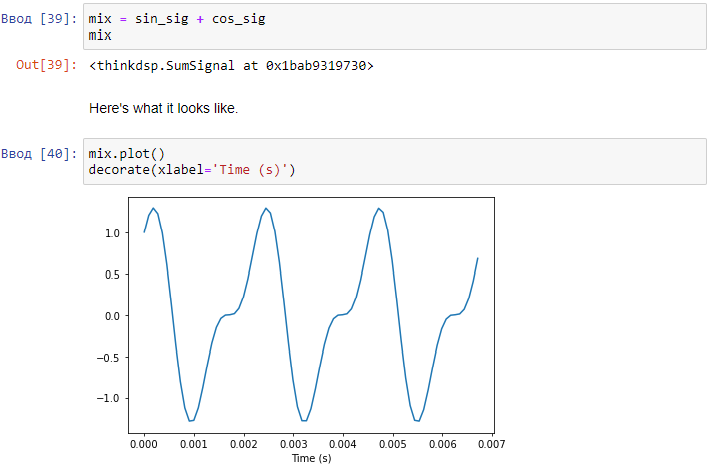
\includegraphics[width=0.65\linewidth]{resources/Images/task1_check1}
        \caption{Изучение и проверка примеров (часть 1).}
        \label{fig:task1_check1}
    \end{figure}

    \begin{figure}[h]
        \centering
        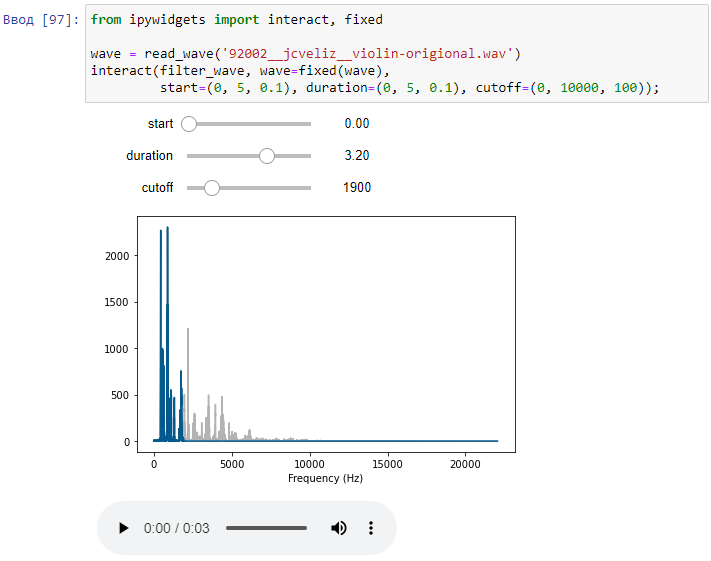
\includegraphics[width=0.65\linewidth]{resources/Images/task1_check2}
        \caption{Изучение и проверка примеров (часть 2).}
        \label{fig:task1_check2}
    \end{figure}

    Как мы видим из Рис.\ref{fig:task1_check1} и Рис.\ref{fig:task1_check2}, все примеры были изучены и запущены.

    \newpage

% ---------------------------------------------- Упражнение 1.2 ----------------------------------------------
    \section{Упражнение 1.2}
    \label{sec:task2}

    Во втором упражнении происходит работа с образцом звука.
    Для этого необходимо скачать с \href{https://freesound.org/}{freesound.org} образец звука, имеющий четко выраженную высоту.
    После этого необходимо выделить полусекундный сегмент с постоянной высотой, вычислить и вывести его спектр.

    Итак, был скачан \href{https://freesound.org/people/tosha73/sounds/509144/}{этот} образец звука с записью школьного звонка.
    Теперь считаем этот файл и выведем его график.
    Для чтения будем использовать \texttt{read\_wave()}, а для построения графика - \texttt{plot()}.

    \begin{lstlisting}[language=Python, caption= Чтение файла звука и вывод графика., label={lst:task2_reading_and_wave}]
        from thinkdsp import read_wave

        wave = read_wave('resources/Sounds/task2_school_rings.wav')
        wave.normalize()
        wave.make_audio()
        wave.plot()
    \end{lstlisting}

    \begin{figure}[h]
        \centering
        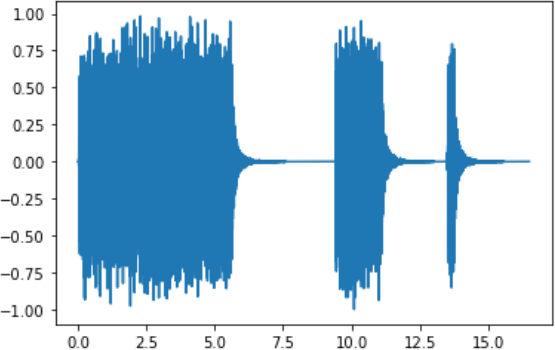
\includegraphics[width=0.8\linewidth]{resources/Images/task2_wave_sound}
        \caption{График образца звука.}
        \label{fig:task2_wave_sound}
    \end{figure}

    Теперь выделим сегмент с постоянной высотой и выведем его график.
    Для выделения сегмента был использован метод \texttt{segment()}.

    \begin{lstlisting}[language=Python, caption= Выделение сегмента и вывод его графика., label={lst:task2_segment}]
        segment = wave.segment(start=5.0, duration=0.3)
        segment.make_audio()
        segment.plot()
    \end{lstlisting}

    \begin{figure}[h]
        \centering
        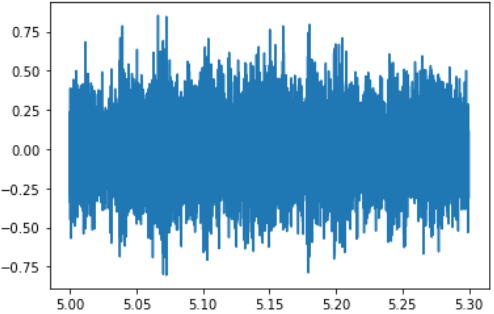
\includegraphics[width=0.8\linewidth]{resources/Images/task2_wave_segment}
        \caption{График сегмента звука.}
        \label{fig:task2_wave_segment}
    \end{figure}

    С помощью \texttt{make\_spectrum()} создадим спектр нашего сегмента.

    \begin{lstlisting}[language=Python, caption= Создание спектра сегмента., label={lst:task2_spectrum}]
        spectrum = segment.make_spectrum()
        spectrum.plot(7000)
    \end{lstlisting}

    \begin{figure}[H]
        \centering
        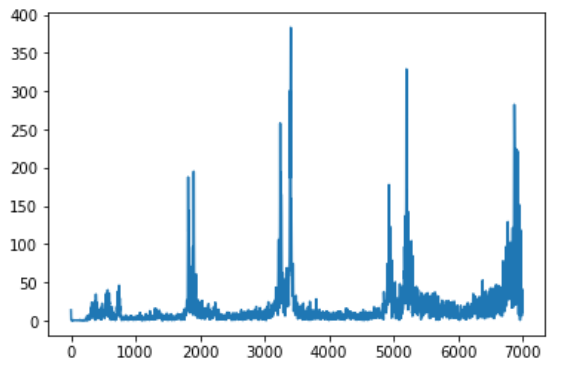
\includegraphics[width=0.8\linewidth]{resources/Images/task2_spectrum}
        \caption{Спектр сегмента записи.}
        \label{fig:task2_spectrum}
    \end{figure}

    Рассмотрим основную и доминирующую частоты, выведем  спектр.

    \begin{lstlisting}[language=Python, caption= Создание спектра сегмента., label={lst:task2_small_spectrum}]
        spectrum.plot(3500)
    \end{lstlisting}

    \begin{figure}[H]
        \centering
        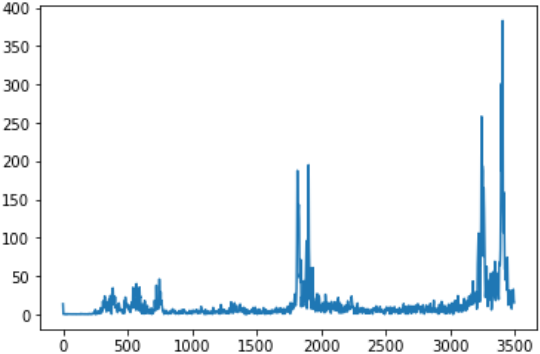
\includegraphics[width=0.7\linewidth]{resources/Images/task2_small_spectrum}
        \caption{Спектр сегмента записи (основная и доминирующая частоты).}
        \label{fig:task2_small_spectrum}
    \end{figure}

    Тембр - это одна из характеристик звука, его "окраска". Тембр зависит от частот в спектре и их интенсивностей.
    Также гармоники образуют тембр.

    Теперь с помощью \texttt{low\_pass()}, \texttt{high\_pass()} и \texttt{band\_stop()} произведём различную фильтрацию и преобразуем спектры обратно в сигнал.

    \begin{lstlisting}[language=Python, caption= Фильтрация гармоник., label={lst:task2_filter}]
        # Filter out the high frequencies
        spectrum.low_pass(2000)
        spectrum.plot(7000)
        spectrum.make_wave().make_audio()

        # Filter out the low frequencies
        spectrum = segment.make_spectrum()
        spectrum.high_pass(2000)
        spectrum.plot(7000)
        spectrum.make_wave().make_audio()

        # Selective filtering
        spectrum = segment.make_spectrum()
        spectrum.band_stop(1500, 6000)
        spectrum.plot(7000)
        spectrum.make_wave().make_audio()
    \end{lstlisting}

    \begin{figure}[H]
        \centering
        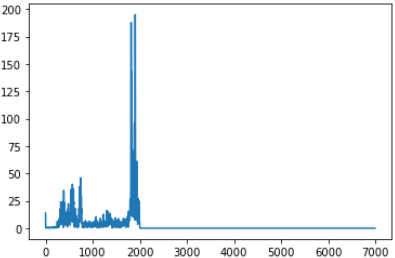
\includegraphics[width=0.8\linewidth]{resources/Images/task2_fiter_low_pass}
        \caption{Спектр, отфильтрованный по высоким частотам.}
        \label{fig:task2_fiter_low_pass}
    \end{figure}

    \begin{figure}[H]
        \centering
        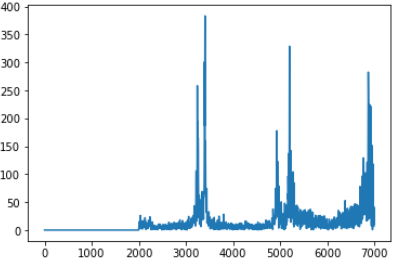
\includegraphics[width=0.8\linewidth]{resources/Images/task2_filter_high_pass}
        \caption{Спектр, отфильтрованный по низким частотам.}
        \label{fig:task2_filter_high_pass}
    \end{figure}

    \begin{figure}[H]
        \centering
        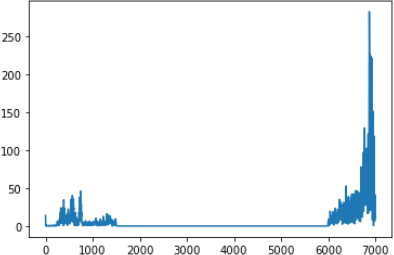
\includegraphics[width=0.8\linewidth]{resources/Images/task2_filter_band_stop}
        \caption{Спектр, отфильтрованный выборочно.}
        \label{fig:task2_filter_band_stop}
    \end{figure}

    Если же прослушать все полученные сигналы, то можно заметить, как отсутствие тех или иных частот влияет на звук.
    Например, отфильтрованный по высоким частотам сигнал вообще не похож на звук школьного звонка.
    Без низких же частот звук становится более сухим и тонким. При выборочной фильтрации звук вообще становится больше похож на стрекот.

    В ходе выполнения данного упражнения была проведена работа с образцом звука.
    Из него был выделен сегмент с постоянной частотой. Был построен его спектр и произведена фильтрация гармоник.
    Полученные в ходе фильтрации спектры были преобразованы обратно в сигналы и прослушаны.

    \newpage

% ---------------------------------------------- Упражнение 1.3 ----------------------------------------------
    \section{Упражнение 1.3}
    \label{sec:task3}

    В этом упражнении нам предстоит создать составной сигнал из объектов \texttt{SinSignal} и \texttt{CosSignal}.
    Затем необходимо обработать сигнал для получения \texttt{wave} и прослушать его, после чего вычислить и построить \texttt{Spectrum}.

    Итак, начнём с создания нескольких экземпляров \texttt{SinSignal} и \texttt{CosSignal}, после чего создадим результирующий сигнал и выведем его на экран.
    Тут же преобразуем его к \texttt{wave} и прослушаем.

    \begin{lstlisting}[language=Python, caption= {Создание сигнала, вывод графика и создание аудио объекта.}, label={lst:task3_plot_signal}]
        from thinkdsp import SinSignal, CosSignal

        sin1 = SinSignal(freq=150, amp=0.5)
        sin2 = SinSignal(freq=800, amp=0.2)
        cos1 = CosSignal(freq=500, amp=0.9)
        cos2 = CosSignal(freq=1000, amp=1.0)

        signal = sin1 + cos1 + sin2 + cos2
        signal.plot()

        wave = signal.make_wave(duration=1)
        wave.make_audio()
    \end{lstlisting}
    \begin{figure}[h]
        \centering
        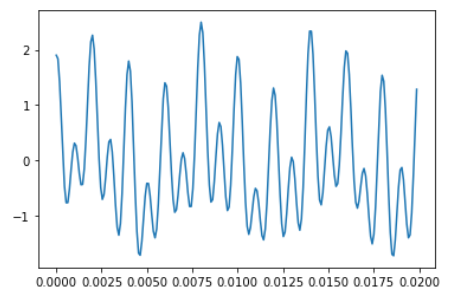
\includegraphics[width=0.7\linewidth]{resources/Images/task3_plot_signal}
        \caption{Составной сигнал.}
        \label{fig:task3_plot_signal}
    \end{figure}

    Получившийся составной сигнал похож на телефонный гудок. Теперь построим спектр и отобразим его.

    \begin{lstlisting}[language=Python, caption= Создание спектра., label={lst:task3_spectrum}]
        spectrum = wave.make_spectrum()
        spectrum.plot(2000)
    \end{lstlisting}

    \begin{figure}[h]
        \centering
        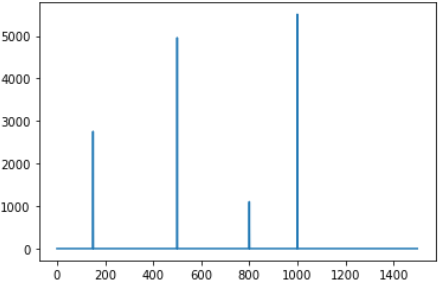
\includegraphics[width=0.8\linewidth]{task3_spectrum}
        \caption{Спектр созданного составного сигнала.}
        \label{fig:task3_spectrum}
    \end{figure}

    Все компоненты, из которых состоит полученный сигнал, кратны 50 Hz, а потому "сливаются" в единый гудок.

    Теперь проверим, что произойдёт, если добавить частотные компоненты, не кратные уже добавленным.
    Для этого прибавим к нашему сигналу ещё по одному \texttt{SinSignal} и \texttt{CosSignal} и прослушаем.

    \begin{lstlisting}[language=Python, caption= Добавление некратных компонент., label={lst:task3_spectrum_update}]
        sin3 = SinSignal(freq=364, amp=0.8)
        cos3 = CosSignal(freq=728, amp=0.7)

        signal2 = signal + sin3 + cos3
        signal2.make_wave(duration=1).make_audio()
    \end{lstlisting}

    В полученном сигнале отчётливо слышны добавленные компоненты, потому что они не кратны 50 Hz.
    Мы слышим их как отдельные высоты, а не как "дополнение" гудка. Кроме того, полученный звук стал менее приятным на слух.

    В ходе выполнения данного упражнения был создан собственный составной сигнал из объектов \texttt{SinSignal} и \texttt{CosSignal}.
    Он был преобразован в \texttt{wave} и прослушан.
    Затем к нему были добавлены некратные компоненты, после чего сигнал снова был прослушан.
    Был сделан вывод, что компоненты, не кратные уже существующим, резко выделяются на фоне остальных.

    \newpage

% ---------------------------------------------- Упражнение 1.4 ----------------------------------------------
    \section{Упражнение 1.4}
    \label{sec:task4}

    Теперь нам необходимо написать функцию \texttt{stretch}, в которую передаётся \texttt{wave} и коэффициент изменения.
    Функция должна ускорять или замедлять сигнал изменением \texttt{ts} и \texttt{framerate}.

    Итак, напишем саму функцию.

    \begin{lstlisting}[language=Python, caption= Описание функции \texttt{stretch}., label={lst:task4_stretch}]
    def stretch(wave_stretch, factor):
        wave_stretch.ts /= factor
        wave_stretch.framerate *= factor
    \end{lstlisting}

    При подаче \texttt{factor} меньше \texttt{1.0} сигнал будет замедляться, если же \texttt{factor} больше \texttt{1.0} - ускоряться.

    Теперь необходимо проверить работу нашей функции.
    Для тестирования будем использовать звуковой файл, который использовался в Упражнении 1.2.
    Для начала создадим два одинаковых \texttt{wave} и прослушаем звук (для удобства сравнения).

    \begin{lstlisting}[language=Python, caption= Считывание звукового файла., label={lst:print_spectrogram}]
        wave1 = read_wave('resources/Sounds/task2_school_rings.wav')
        wave2 = wave1
        wave1.make_audio()
    \end{lstlisting}

    Теперь замедлим один сигнал и ускорим второй, прослушаем результат и выведем графики сигналов.

    \begin{lstlisting}[language=Python, caption= Редактирование сигналов с помощью \texttt{factor}., label={lst:editing_signals}]
        # Deceleration
        stretch(wave1, 0.3)
        wave1.make_audio()
        wave1.plot()
        # Acceleration
        stretch(wave2, 5.0)
        wave2.make_audio()
        wave2.plot()
    \end{lstlisting}

    Замедленный звук стал более низким и менее резким. Ускоренный же звук наоборот стал более звонким, высоким и резким.
    При сравнении полученных графиков с графиком нетронутого звука (Рис.\ref{fig:task2_wave_sound}) можно заметить, что ускоренный сигнал сжался, а замеленный - растянулся.

    \begin{figure}[H]
        \centering
        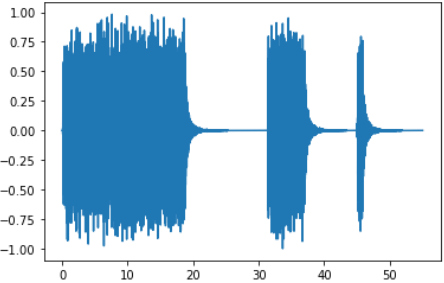
\includegraphics[width=0.7\linewidth]{task4_signal_deceleration}
        \caption{Замедленный сигнал.}
        \label{fig:task4_signal_deceleration}
    \end{figure}

    \begin{figure}[H]
        \centering
        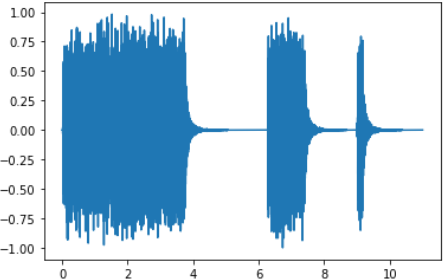
\includegraphics[width=0.7\linewidth]{task4_signal_acceleration}
        \caption{Ускоренный сигнал.}
        \label{fig:task4_signal_acceleration}
    \end{figure}

    Исходя из результатов тестирования, можно сделать вывод, что написанная функция \texttt{stretch} работает корректно.

    В ходе выполнения данного упражнения была написана функция \texttt{stretch}.
    Она принимает на вход \texttt{wave} и коэффициент изменения.
    Функция ускоряет или замедляет сигнал (в зависимости от поданного \texttt{factor}) изменением \texttt{ts} и \texttt{framerate}.
    Функция была протестирована, и был сделан вывод, что она работает корректно.

    \newpage

% ------------------------------------------------- Выводы -------------------------------------------------
    \section{Выводы}
    \label{sec:conclusions}

    В ходе выполнения данной лабораторной работы были изучены объекты Signal, Wave и Spectrum.
    Также были получены навыки по работе с сигналами, их обработке и фильтрации, созданию спектров и собственных составных сигналов.
    Кроме того, были получены знания о том, как именно небольшое конкретное изменение сигнала может повлиять на звук.

\end{document}